\documentclass{article}
\usepackage{amsmath}
\usepackage{graphicx}
\usepackage{hyperref}
\usepackage{listings}
\usepackage{xcolor}
\usepackage{tikz}
\usetikzlibrary{automata,positioning}

\definecolor{codegreen}{rgb}{0,0.6,0}
\definecolor{codegray}{rgb}{0.5,0.5,0.5}
\definecolor{codepurple}{rgb}{0.58,0,0.82}
\definecolor{backcolour}{rgb}{0.95,0.95,0.92}

\lstdefinestyle{mystyle}{
    backgroundcolor=\color{backcolour},
    commentstyle=\color{codegreen},
    keywordstyle=\color{magenta},
    numberstyle=\tiny\color{codegray},
    stringstyle=\color{codepurple},
    basicstyle=\ttfamily\footnotesize,
    breakatwhitespace=false,
    breaklines=true,
    captionpos=b,
    keepspaces=true,
    numbers=left,
    numbersep=5pt,
    showspaces=false,
    showstringspaces=false,
    showtabs=false,
    tabsize=2
}

\lstset{style=mystyle}

\title{Structured Output with Large Language Models}
\author{AI Research Team}
\date{\today}

\begin{document}

\maketitle

\begin{abstract}
Large Language Models (LLMs) excel at generating human-like text but face challenges when required to produce structured output in a consistent manner. This article explores the need for structured output in LLM applications, the challenges involved, and various techniques for ensuring that LLMs generate output in specific formats. We examine prompt engineering, fine-tuning approaches, and logit post-processing methods, along with practical tools for implementing these techniques.
\end{abstract}

\section{Introduction}

While Language Models excel at generating human-like text, they face challenges when tasked with producing structured output in a consistent manner. This limitation becomes particularly problematic when integrating LLMs into production systems that require well-formatted data for downstream processing through databases, APIs, or other software applications. Even carefully crafted prompts cannot guarantee that an LLM will maintain the expected structure throughout its response.

User needs driving the demand for LLM output constraints can be broadly categorized as follows:

\subsection{Improving Developer Efficiency and Workflow}
\begin{itemize}
    \item \textbf{Reducing Trial and Error in Prompt Engineering:} Developers find the process of crafting prompts to elicit desired output formats to be time-consuming, often involving extensive testing and iteration. LLM output constraints could make this process more efficient and predictable.
    \item \textbf{Minimizing Post-processing of LLM Outputs:} Developers frequently have to write complex code to wrangle and process LLM outputs that don't conform to expected formats. LLM structured output would simplify this, reducing the need for ad-hoc post-processing code.
    \item \textbf{Streamlining Integration with Downstream Processes:} LLMs are often used within larger pipelines where their output serves as input for subsequent modules. Output constraints are crucial to ensure compatibility and prevent errors.
    \item \textbf{Enhancing the Quality of Synthetic Datasets:} LLMs are increasingly used to generate synthetic data for AI training. Constraints can ensure data integrity and prevent the inclusion of unwanted elements that could negatively impact training outcomes.
\end{itemize}

\subsection{Meeting UI and Product Requirements}
\begin{itemize}
    \item \textbf{Adhering to UI Size Limitations:} LLM-generated content often needs to fit into specific UI elements with size restrictions, especially on mobile devices. Output length constraints prevent content overflow and ensure proper display within the UI.
    \item \textbf{Ensuring Output Consistency:} Consistent output length and format are crucial for user experience and UI clarity. Constraints help maintain this consistency, avoiding overwhelming variability in generated text.
    \item \textbf{Complying with Platform Character Limits:} Certain platforms, such as Twitter or YouTube Shorts, impose character limits on content. Length constraints allow LLMs to comply with these restrictions, ensuring content can be published successfully.
\end{itemize}

\subsection{Enhancing User Trust and Experience}
\begin{itemize}
    \item \textbf{Improving Reliability:} Structured output ensures that LLM responses are reliable and predictable, enhancing user trust in the system.
    \item \textbf{Facilitating Automated Processing:} When LLM outputs need to be processed by other systems, structured formats like JSON or XML make this integration seamless.
\end{itemize}

\section{Problem Statement}

Language models based on the Transformer architecture are next token prediction machines. These models calculate the probability of observing a token (from a vocabulary of size $n$) conditioned on the previous tokens in the sequence. This process can be expressed mathematically as:

$$P(x_i | x_{<i})$$

where, $x_i$ represents the current token being generated, while $x_{<i}$ encompasses all preceding tokens.

However, in practical applications, generating high-quality content requires more than just probabilistic next-token generation. The key challenge lies in incorporating control conditions ($C$) that guide the model to produce text with specific desired characteristics - whether that's maintaining a consistent format, following syntactic rules, or adhering to semantic constraints. These control conditions must be integrated while preserving the model's ability to generate natural, coherent text. This controlled text generation process can be formalized as:

$$P(x_i | x_{<i}, C)$$

Here, $C$ represents the set of constraints or control conditions that shape the generated output. Common constraints include:

\begin{itemize}
    \item \textbf{Format Constraints:} Enforcing specific output formats like JSON, XML, or YAML ensures the generated content follows a well-defined structure that can be easily parsed and validated.
    \item \textbf{Multiple Choice Constraints:} Restricting LLM outputs to a predefined set of options helps ensure valid responses and reduces the likelihood of unexpected or invalid outputs.
    \item \textbf{Static Typing Constraints:} Enforcing data type requirements (strings, integers, booleans, etc.) ensures outputs can be safely processed by downstream systems.
    \item \textbf{Length Constraints:} Limiting the length of generated content is crucial for UI display, platform requirements, and maintaining consistent user experience.
\end{itemize}

\section{Techniques for Structured Output}

There are many techniques to obtain structured output from LLMs. They can be broadly categorized into two types based on the phase they are applied to:

\begin{itemize}
    \item \textbf{Training-Time Techniques (TTT):} These techniques are applied during the training or post-training phases of the LLM. They are used to guide the model to learn the specific patterns and structures that are required for the task at hand.
    \item \textbf{Inference-Time Techniques (ITT):} These techniques are applied during the inference phase of the LLM. They are used to guide the model to produce the desired output at inference time.
\end{itemize}

Within these two broad categories, the most common approaches are (in decreasing order of popularity but increasing order of reliability):

\subsection{Prompt Engineering (ITT)}

Prompt engineering is a technique that involves crafting a prompt to guide the LLM to produce the desired output. This can be achieved by using tools like Pydantic to define the expected data structure and then using that definition to guide the LLM's output.

Perhaps the most common strategy to generate LLM response in a target format is using one-shot prompting, where the user provides an example of the desired output format within the prompt.

As a motivating example, consider the following simple task: Given a segment of a SEC financial filing, generate a two-person discussion about key financial data from the text in JSON format, simulating what would be a real-world discussion about the underlying companies' disclosed financial information.

\begin{lstlisting}[language=Python, caption=One-shot prompting for structured output]
prompt = """
Generate a two-person discussion about the key financial data from the following text in JSON format.

<JSON_FORMAT>
{
   "Person1": {
     "name": "Alice",
     "statement": "The revenue for Q1 has increased by 20% compared to last year."
   },
   "Person2": {
     "name": "Bob",
     "statement": "That's great news! What about the net profit margin?"
   }
}
</JSON_FORMAT>
"""

response = client.chat.completions.create(
    model="gpt-4o-mini",
    messages=[
        {"role": "system", "content": prompt},
        {"role": "user", "content": sec_filing}
    ]
)
\end{lstlisting}

While this approach is simple, it may not be sufficient for complex (e.g., nested) structures and/or when the model's output needs to be restricted to a specific set of options or types.

\subsection{JSON Mode (Fine-Tuned)}

Some models offer "JSON Mode" as an attempt to handle those challenges. This is a feature provided by most LLM API providers today, such as OpenAI, that allows the model to generate output in JSON format. This is particularly useful when you need structured data as a result, such as when parsing the output programmatically or integrating it with other systems that require JSON input.

\begin{lstlisting}[language=Python, caption=Using JSON mode with OpenAI API]
prompt = f"""
Generate a two-person discussion about the key financial data from the following text in JSON format.
TEXT: {sec_filing}
"""
response = client.chat.completions.create(
    model="gpt-3.5-turbo",
    messages=[{"role": "user", "content": prompt}],
    response_format = { "type": "json_object" }
)
\end{lstlisting}

JSON mode is typically a form of fine-tuning, where a base model went though a post-training process to learn target formats. However, while useful this strategy is not guaranteed to work all the time.

In addition to JSON mode, "Structured Output" mode is also becoming popular among LLM providers. This is a feature that ensures the model will always generate responses that adhere to your supplied JSON Schema. Some benefits include:

\begin{itemize}
    \item Reliable type-safety: No need to validate or retry incorrectly formatted responses.
    \item Explicit refusals: Safety-based model refusals are now programmatically detectable.
    \item Simpler prompting: No need for strongly worded prompts to achieve consistent formatting.
\end{itemize}

\subsection{Logit Post-Processing (ITT)}

Logit post-processing is a technique that involves modifying the logits of the LLM's output before it is converted into text such that we have a "controlled" text generation.

The text generation process follows a probabilistic approach. At each step, the model calculates the probability distribution over its entire vocabulary to determine the most likely next token.

The main idea here is that we can modify the logits of the last token to bias the model towards the tokens we want to see in the output hence "controlling" the generation process.

\begin{figure}
    \centering
    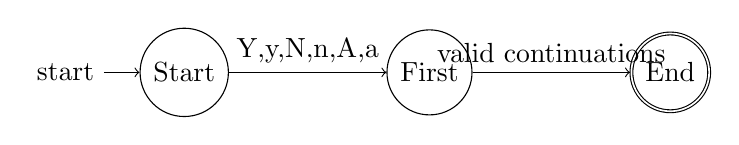
\begin{tikzpicture}[node distance=2cm, auto]
        \node[state, initial] (S) {Start};
        \node[state, right=of S] (F) {First};
        \node[state, right=of F, accepting] (E) {End};
        \path[->] (S) edge node {Y,y,N,n,A,a} (F);
        \path[->] (F) edge node {valid continuations} (E);
    \end{tikzpicture}
    \caption{Simplified state machine for logit post-processing}
    \label{fig:state-machine}
\end{figure}

The transformers library provides a LogitsProcessor class that allows us to modify the logits of the last token. With logit processing, we can modify the logits to bias the model towards the tokens we want to see in the output.

\section{Tools for Structured Output}

\subsection{Outlines}

Outlines is a library specifically focused on structured text generation from LLMs. Under the hood, Outlines works by adjusting the probability distribution of the model's output logits - the raw scores from the final layer of the neural network that are normally converted into text tokens. By introducing carefully crafted logit biases, Outlines can guide the model to prefer certain tokens over others, effectively constraining its outputs to a predefined set of valid options.

The authors solve the general guided generation problem, which, as a consequence, solves the problem of structured output generation in LLMs by introducing an efficient indexing approach that reformulates neural text generation using finite-state machines (FSMs).

Outlines provides several powerful controlled generation features for developers:
\begin{itemize}
    \item Regex-based structured generation: Guide the generation process using regular expressions.
    \item Multiple Choice Generation: Restrict the LLM output to a predefined set of options.
    \item Pydantic model: Ensure the LLM output follows a Pydantic model.
    \item JSON Schema: Ensure the LLM output follows a JSON Schema.
\end{itemize}

\begin{lstlisting}[language=Python, caption=Using Outlines for multiple choice generation]
import outlines

model = outlines.models.transformers("Qwen/Qwen2.5-0.5B-Instruct")

prompt = """You are a sentiment-labelling assistant specialized in Financial Statements.
Is the following document positive or negative?

Document: {document_text}
"""

generator = outlines.generate.choice(model, ["Positive", "Negative"])
answer = generator(prompt)
print(answer)
\end{lstlisting}

\subsection{LangChain}

LangChain is a framework designed to simplify the development of LLM applications. It provides an abstraction layer over many LLM providers that in turn offers structured output.

In particular, LangChain offers the with\_structured\_output method, which can be used with LLMs that support structured output APIs, allowing you to enforce a schema directly within the prompt.

\begin{lstlisting}[language=Python, caption=Using LangChain for structured output]
from langchain_openai import ChatOpenAI
from langchain_core.prompts import ChatPromptTemplate

def extract_structured_data(input_text: str, prompt: str):
    llm = ChatOpenAI(model="gpt-4o-mini")
    structured_llm = llm.with_structured_output(DataModel)
    
    prompt_template = ChatPromptTemplate.from_messages(
        [
            ("system", prompt),
            ("human", "{input_text}"),
        ]
    )

    llm_chain = prompt_template | structured_llm
    return llm_chain.invoke(input_text)
\end{lstlisting}

\subsection{Ollama}

Ollama is a tool for running open-source large language models locally. It provides a simple API for generating structured output from LLMs. Ollama supports JSON mode for models that have been fine-tuned for structured output.

\section{Best Practices for Structured Output}

When working with structured output in LLMs, consider the following best practices:

\begin{itemize}
    \item \textbf{Define Clear Schemas:} Provide clear and detailed schemas for the expected output format. This helps the model understand the structure you want.
    \item \textbf{Use Examples:} Provide examples of the expected output format in your prompts. This helps the model understand the structure you want.
    \item \textbf{Validate Outputs:} Always validate the model's outputs to ensure they conform to the expected structure. This is especially important for critical applications.
    \item \textbf{Handle Failures Gracefully:} Have fallback mechanisms in place for when the model fails to produce the expected structured output.
    \item \textbf{Consider Model Capabilities:} Different models have different capabilities when it comes to structured output. Choose the right model for your task.
\end{itemize}

\section{Conclusion}

Structured output generation is a critical capability for integrating LLMs into production systems. Various techniques and tools are available to ensure that LLMs generate output in specific formats, from simple prompt engineering to more sophisticated approaches like logit post-processing.

The choice of technique depends on the specific requirements of the application, the complexity of the desired output structure, and the capabilities of the available models. By understanding these techniques and tools, developers can effectively leverage LLMs for a wide range of applications that require structured data.

\section{References}

\begin{enumerate}
    \item Liang, P., et al. (2024). Holistic Evaluation of Language Models. arXiv preprint arXiv:2211.09110.
    \item Liu, J., et al. (2024). The Need for Constraints on Large Language Models. Google Research.
    \item NousResearch. (2024). Hermes-2-Theta-Llama-3-8B. https://huggingface.co/NousResearch/Hermes-2-Theta-Llama-3-8B
    \item Outlines. (2024). Outlines: Structured Generation with LLMs. https://github.com/outlines-dev/outlines
    \item Shorten, C., et al. (2024). Structured Output for Large Language Models. arXiv preprint arXiv:2401.12443.
    \item Tang, Y., et al. (2024). Structured Prompting for Large Language Models. arXiv preprint arXiv:2402.10949.
    \item Tran-Thien, L. (2024). Outlines: Guided Generation with LLMs. https://outlines-dev.github.io/outlines/
    \item Willard, B., & Louf, J. (2023). Guided Generation: Constrained Decoding for LLMs. arXiv preprint arXiv:2307.09702.
\end{enumerate}

\end{document}
